%!TeX root=../tese.tex
%("dica" para o editor de texto: este arquivo é parte de um documento maior)
% para saber mais: https://tex.stackexchange.com/q/78101

%% ------------------------------------------------------------------------- %%

% "\chapter" cria um capítulo com número e o coloca no sumário; "\chapter*"
% cria um capítulo sem número e não o coloca no sumário. A introdução não
% deve ser numerada, mas deve aparecer no sumário. Por conta disso, este
% modelo define o comando "\chapter**".
\chapter**{Introdução}
\label{cap:introducao}

\enlargethispage{.5\baselineskip}

O ensino da computação estimula o desenvolvimento de importantes habilidades
do mundo digital, como o raciocínio lógico, a análise e resolução de problemas,
o pensamento crítico, a criatividade, a colaboração, entre outras. O pensamento
computacional, que possibilita o desenvolvimento dessas habilidades, vai muito
além de programar, sendo fundamental não somente para ciência da computação,
mas também para leitura, escrita e aritmética, proporcionando capacidades
analíticas para crianças \citep{wing2006computational}.

%%%%%%%%%%%%%%%%%%%%%%%%%%%%%%%%%%%%%%%%%%%%%%%%%%%%%%%%%%%%%%%%%%%%%%%%%%%%%%%
%% Algumas delas também estão envolvidas no conceito de pensamento computacional, o qual vai muito além de programar, mas requer múltiplos níveis de abstração, sendo a forma como humanos resolvem problemas, tendo como base a matemática \citet{wing2006computational}. 
%%%%%%%%%%%%%%%%%%%%%%%%%%%%%%%%%%%%%%%%%%%%%%%%%%%%%%%%%%%%%%%%%%%%%%%%%%%%%%%

Essas habilidades são cada vez mais relevantes para crianças e jovens de diversas faixas etárias. Nesse sentido, muito tem sido discutido acerca da aprendizagem de computação na educação básica nas últimas décadas. Escolas em vários países ao redor do mundo já introduziram o ensino de computação. Alguns estudos revelam os desafios e as expectativas desta implementação, além de fatores importantes na educação, em escolas k-12, as quais correspondem às séries do jardim de infância ao ensino médio.

\citet{hubwieser2015global} mostraram a situação do ensino de computação em escolas k-12 em 14 casos de estudo em estados de 12 países: Alemanha, Estados Unidos, Índia, Nova Zelândia, França, Coreia, Suécia, Reino Unido, Finlândia, Israel, Rússia e Itália. Eles identificaram diferenças em diversos aspectos nas abordagens, encontrando cerca de 40 termos diferentes para descrever áreas relacionadas à ciência da computação, 24 categorias de objetivos de ensino e 19 de conteúdos de computação, 4 subcategorias de linguagens de programação (sistemas baseados em hardware, ambientes de programação educacional com linguagem própria e baseados em outras linguagens, e linguagens de programação profissionais), e diferentes níveis de educação exigidos dos professores. Os autores acreditam que o mapeamento realizado pode contribuir no processo de planejamento do currículo de ciência da computação nas escolas de ensino fundamental e que a computação poderá se tornar uma matéria regular na educação básica em todos os países do mundo.

Outro trabalho, conduzido por \citet{falkner2019international}, analisou a implementação do ensino de ciência da computação no k-12, comparando os requisitos curriculares definidos por padrões (pretendido) com o que realmente é implementado nas salas de aula pelos docentes. Foram analisados currículos em 7 países: Austrália, Inglaterra, Irlanda, Itália, Malta, Escócia e Estados Unidos, com foco apenas em conceitos de ciência da computação e linguagens de programação. Eles observaram que os tópicos mais ensinados são algoritmos, programação, pensamento computacional e representação de dados. Alguns tópicos, como inteligência artificial e robótica, constam no currículo pretendido de apenas um país cada, mas são abordados em sala de aula em diversos países. Ainda, eles descobriram que os educadores tendem a escolher as linguagens de programação baseados em fatores motivados pelos alunos ao invés de se basearem no currículo pretendido. O estudo mostrou que os professores utilizam tanto programação visual quanto baseada em texto no ensino fundamental, além de identificarem o uso comum de atividades desplugadas, apesar destas não estarem explicitamente definidas no currículo padrão. Os autores também identificaram diferenças no alinhamento curricular entre os países, as quais acreditam que possam ajudar a guiar uma futura reforma curricular.

Ademais, \citet{zhu2023core} realizaram uma pesquisa fenomenológica sobre fatores críticos na educação de ciência da computação em escolas k-12, a partir das perspectivas e visões de professores do ensino superior e de k-12. As entrevistas semi-estruturadas conduzidas com os docentes indicaram que as habilidades de resolução de problemas pelos estudantes, através do pensamento computacional, são as competências mais importantes no ensino de computação no k-12. Além disso, conhecimentos básicos em matemática e programação também são bastante relevantes, enquanto que o ensino de linguagens de programação específicas não foram consideradas importantes.

No Brasil, pesquisadores, instituições de ensino e organizações juntaram esforços para implementar o ensino de computação na educação básica. Segundo relatório do Conselho Nacional de Educação (CNE) \citep{brasil2021normas}, com a implantação da Base Nacional Comum Curricular (BNCC) em 2017, o CNE ficou responsável por elaborar as normas específicas sobre computação. Entre 2019 e 2021, foram designados os membros da comissão para formular tais normas. Também houve colaborações de pesquisadores da Sociedade Brasileira de Computação (SBC), do Centro de Inovação para a Educação Brasileira (CIEB), do Ministério da Educação (MEC), dentre outras organizações. Finalmente, em 2022, o CNE homologou as Normas sobre Computação na Educação Básica - Complemento à Base Nacional Comum Curricular (BNCC). Alguns estudos mostram o panorama do processo de implementação da computação na educação básica brasileira.

\citet{defranca2013ensino} realizaram um mapeamento sistemático de artigos referentes ao ensino de computação na educação básica publicados entre os anos de 2009 e 2012. Eles observaram um crescente interesse dos pesquisadores brasileiros no assunto, com destaque para as instituições de pesquisa das regiões Nordeste e Sul do país. Em outro estudo, \citet{bordini2016computaccao} apresentaram um levantamento de trabalhos relacionados ao pensamento computacional no ensino fundamental e médio realizados entre 2010 e 2015, com o intuito de mostrar o que já foi alcançado nessa área no Brasil. Eles identificaram diferenças nas metodologias de ensino, bem como nas ferramentas utilizadas e no público alvo dos estudos, mostrando conformidade com os trabalhos internacionais.

Ainda, \citet{santos2018mapping} analisaram a literatura sobre pensamento computacional e programação na educação básica brasileira no período de 2001 a 2016.  Eles consideraram fatores como metodologia, ferramentas, público alvo e outros, mostrando novamente o crescente interesse dos pesquisadores no tema. Ademais, os autores apontaram algumas tendências e lacunas nessa área. \citet{dossantos2021ensinar} realizaram uma revisão sistemática sobre as diferentes abordagens de ensino de computação no ensino fundamental em estudos publicados entre 2009 e 2020, em bases nacionais e internacionais. Eles analisaram diferentes tipos de atividades voltadas ao ensino de computação: plugadas, desplugadas e híbridas, apontando tendências e lacunas observadas nos trabalhos, como por exemplo, equidade e inclusão.

Diante desse cenário nacional e mundial, a SBC elaborou as Diretrizes de Ensino de Computação na Educação Básica \citep{ribeiro2019diretrizes}, visando facilitar a implementação do ensino de computação nos currículos das escolas brasileiras. Os conceitos de Computação são organizados em 3 eixos, como mostra a Figura 1:

\begin{itemize}
    \item Pensamento Computacional: refere-se à habilidade de analisar, compreender, modelar, comparar, solucionar e automatizar problemas e soluções de maneira sistemática, por meio de abstrações, análise de informações e da construção de algoritmos. 
    \item Mundo Digital: nele ocorre a codificação ou representação de informações, o processamento dos dados codificados e a distribuição dessas informações de forma segura.
    \item Cultura Digital: envolve o conhecimento das tecnologias digitais, bem como as relações da computação com outras áreas do conhecimento e a participação crítica, ética e responsável na sociedade do Mundo Digital.
\end{itemize}

\begin{figure}[h!]
    \centering
    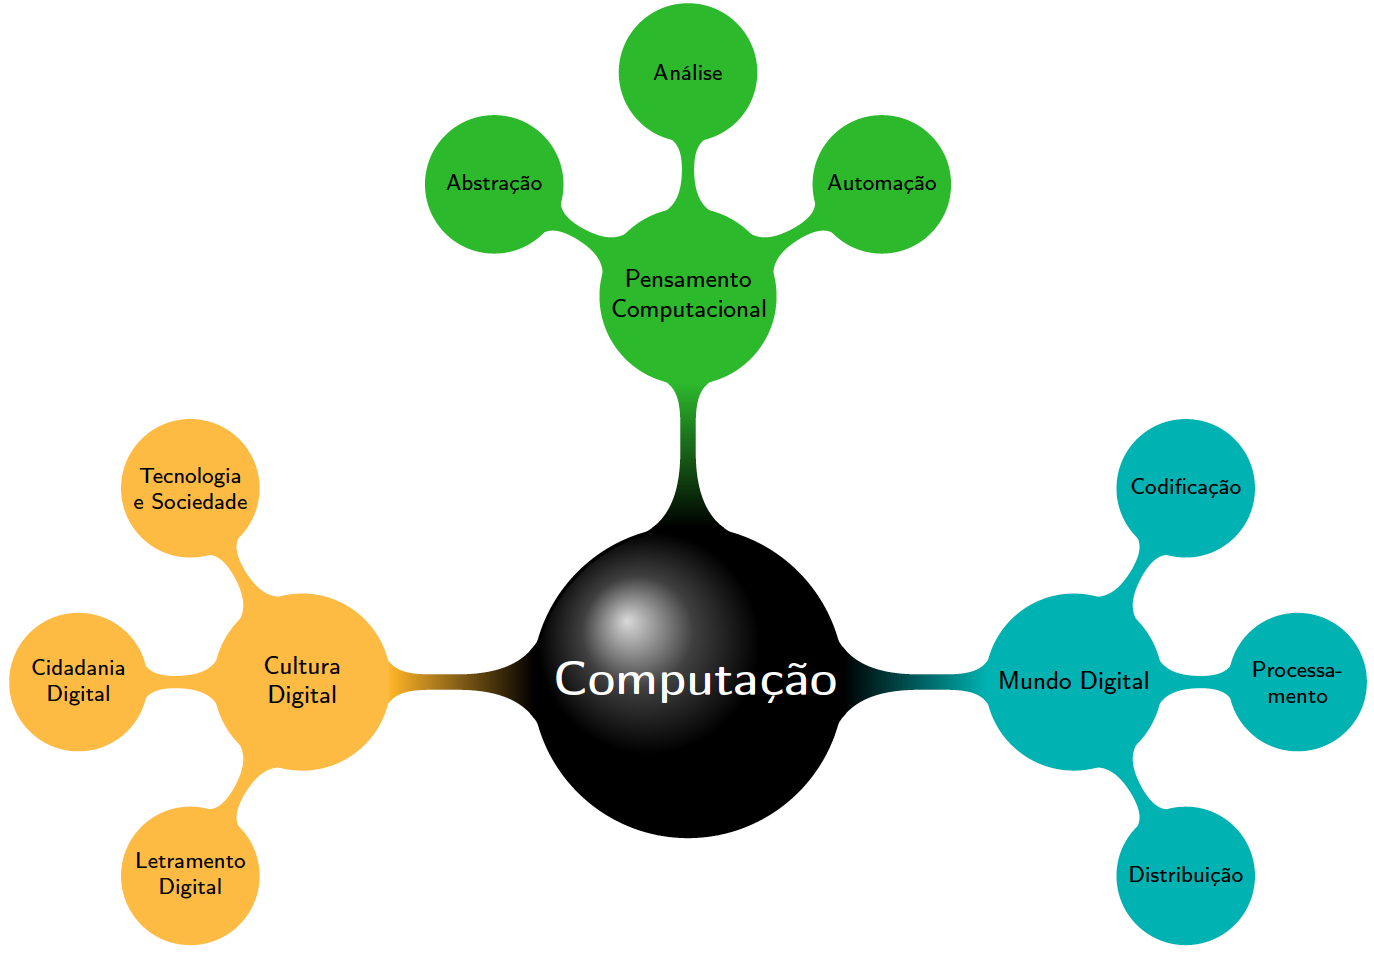
\includegraphics[scale=0.25]{eixos_computacao.png}
    \caption{Eixos da Computação \citep{ribeiro2019diretrizes}.}
    \label{figure:eixos_computacao}
\end{figure}

Dessa forma, é possível perceber que o ensino de computação não se limita à aprendizagem de uma linguagem de programação. Ela é apenas uma ferramenta utilizada para aplicar estes conceitos de forma a chegar na solução de problemas, a partir do conhecimento de teoria da computação e paradigmas de programação \citep{blatt2017mapeamento}. Assim, diferentes metodologias podem ser adotadas no ensino de programação para crianças e jovens e o uso de recursos didáticos apropriados, ferramentas ou aplicativos pedagógicos, é indispensável no aprendizado desses conceitos.

Há diversas maneiras de explorar a aprendizagem dos conceitos de computação: jogos, programação visual, programação com blocos, kits de robótica, simulações, storytelling, entre outras. Dentre as ferramentas utilizadas no ensino fundamental, nota-se uma preferência pelas linguagens visuais e plataformas focadas no ensino dos fundamentos e não no desenvolvimento \citep{gomes2017ensino}. A linguagem de programação em blocos é uma das mais citadas em estudos, apresentando diversas opções de ferramentas \citep{brezolin2021panorama,desouza2021ensino}. 

Deste modo, softwares de apoio ao ensino de programação devem facilitar a compreensão das abstrações envolvidas nos conceitos de computação, bem como, estimular o raciocínio lógico. Nesse sentido, o uso de simulações interativas facilita a visualização de conceitos abstratos, utilizando exemplos concretos para representá-los. 

%% capítulo de ferramnetas
% \citet{fernandes2012animaccoes} obtiveram resultados positivos na criação de objetos de aprendizagem na forma de animações e simulações em temas de lógica de programação, demonstrando o potencial dessa ferramenta.

Alguns trabalhos mostram a efetividade das simulações no ensino em outras áreas. Em particular, a plataforma de simulações interativas PhET (Physics Education Technology) é um recurso bastante utilizado em várias disciplinas de ciências \citep{khatri2013over}. Criado em 2002 pelo ganhador do prêmio Nobel, Carl Wieman, o projeto da Universidade de Colorado Boulder apresenta atualmente 159 simulações interativas distribuídas nas áreas de física, química, matemática, ciências da terra e biologia, destinadas tanto a alunos da educação básica como de ensino superior.

Entre 2012 e 2013, a plataforma realizou uma pesquisa com docentes que utilizavam a ferramenta, recebendo cerca de 2000 respostas de escolas nos Estados Unidos \citep{price2018and}. O estudo mostrou três aspectos que contribuem para a escolha da ferramenta na sala de aula. Primeiro, devido a sua flexibilidade, as simulações são utilizadas de diversas maneiras e com diferentes objetivos de aprendizagem, como entender conceitos, processos científicos e aumentar a motivação dos estudantes. Além disso, os docentes preferem que os estudantes tenham controle da simulação. Por fim, algumas propriedades percebidas das simulações foram a visualização, manipulabilidade e a capacidade de realizar demonstrações que não poderiam ser feitas em sala.

No Brasil, diversos estudos mostram pontos positivos da utilização dessa ferramenta como forma de agregar ao ensino tradicional. Uma pesquisa bibliográfica de publicações de autores brasileiros entre os anos de 2010 e 2020, realizada por \citet{ramos2020ensino}, mostrou que a utilização do simulador PhET, junto a uma metodologia de ensino, potencializou o aprendizado dos estudantes, além de torná-los participantes ativos desse processo.

Outro trabalho, conduzido por \citet{cravo2021avaliaccao}, reforça esta conclusão. Eles avaliaram simulações de ciências e biologia, através de um protocolo de avaliação próprio e da realização de oficinas com futuros docentes, mostrando os desafios e potencialidade da ferramenta. Os autores concluíram que ela contribui positivamente no processo de ensino-aprendizagem, tornando-o mais didático e dinâmico,  e que a atuação de professores como mediadores do ensino pode ajudar a contornar possíveis deficiências na sua utilização. Ainda, os trabalhos de \citet{araujo2021uso,santos2020revisao} apresentam conclusões similares em relação ao uso de simulações no ensino de física e química, respectivamente.

Assim, esta é uma abordagem interessante a ser explorada também no ensino da computação, pois da mesma forma que as ciências da natureza e das humanidades ajudam a explicar o mundo real, a ciência da computação ajuda a explicar o mundo digital \citep{ribeiro2019diretrizes}. Portanto, é natural que busquemos ferramentas análogas para o estudo dessas ciências, e até onde sabemos, não existem simulações de conceitos de lógica de programação iguais às encontradas no PhET.

Desse modo, este projeto de pesquisa tem como objetivo a criação de um produto mínimo viável (MVP - \textit{Minimum Viable Product}) de uma ferramenta de simulações interativas para o ensino de conceitos de lógica de programação para crianças no ensino fundamental. Para isso, iremos desenvolver uma versão da aplicação com um conjunto mínimo de requisitos, contendo uma simulação que envolva alguns conceitos de lógica de programação. Além disso, queremos que os usuários tenham contato com a estrutura real do código de programação correspondente a cada conceito simulado. Assim, pretendemos integrar à simulação uma visualização do pseudocódigo associado.

Também queremos aplicar o MVP em sala de aula para obter \textit{feedback} para um futuro desenvolvimento do sistema completo. Dessa forma, iremos avaliar a sua usabilidade com a ajuda de estudantes do ensino fundamental, através de um questionário de usabilidade. Ademais, queremos investigar como representar os conceitos visualmente de forma que facilite a compreensão da lógica de programação por trás deles.
